%% whole_genome_alignment.tex
%% Author: Leighton Pritchard
%% Copyright: James Hutton Institute
%% A brief description of whole genome alignment and comparison


% SUBSECTION: Whole genome alignments
\subsection{An Introduction to Whole Genome Alignment}

% What do you align, and why?
\begin{frame}
  \frametitle{What to align, and why?}
  For useful analysis, the aligned genomes should:
  \begin{itemize}
    \item derive from a sufficiently recent common ancestor, so homologous regions can be identified
    \item derive from a sufficiently distant common ancestor, so that there are ``interesting'' differences to be identified
    \item \textbf{help to answer your biological question}: is your question organism or phenotype-specific? 
  \end{itemize}
  \begin{center}
    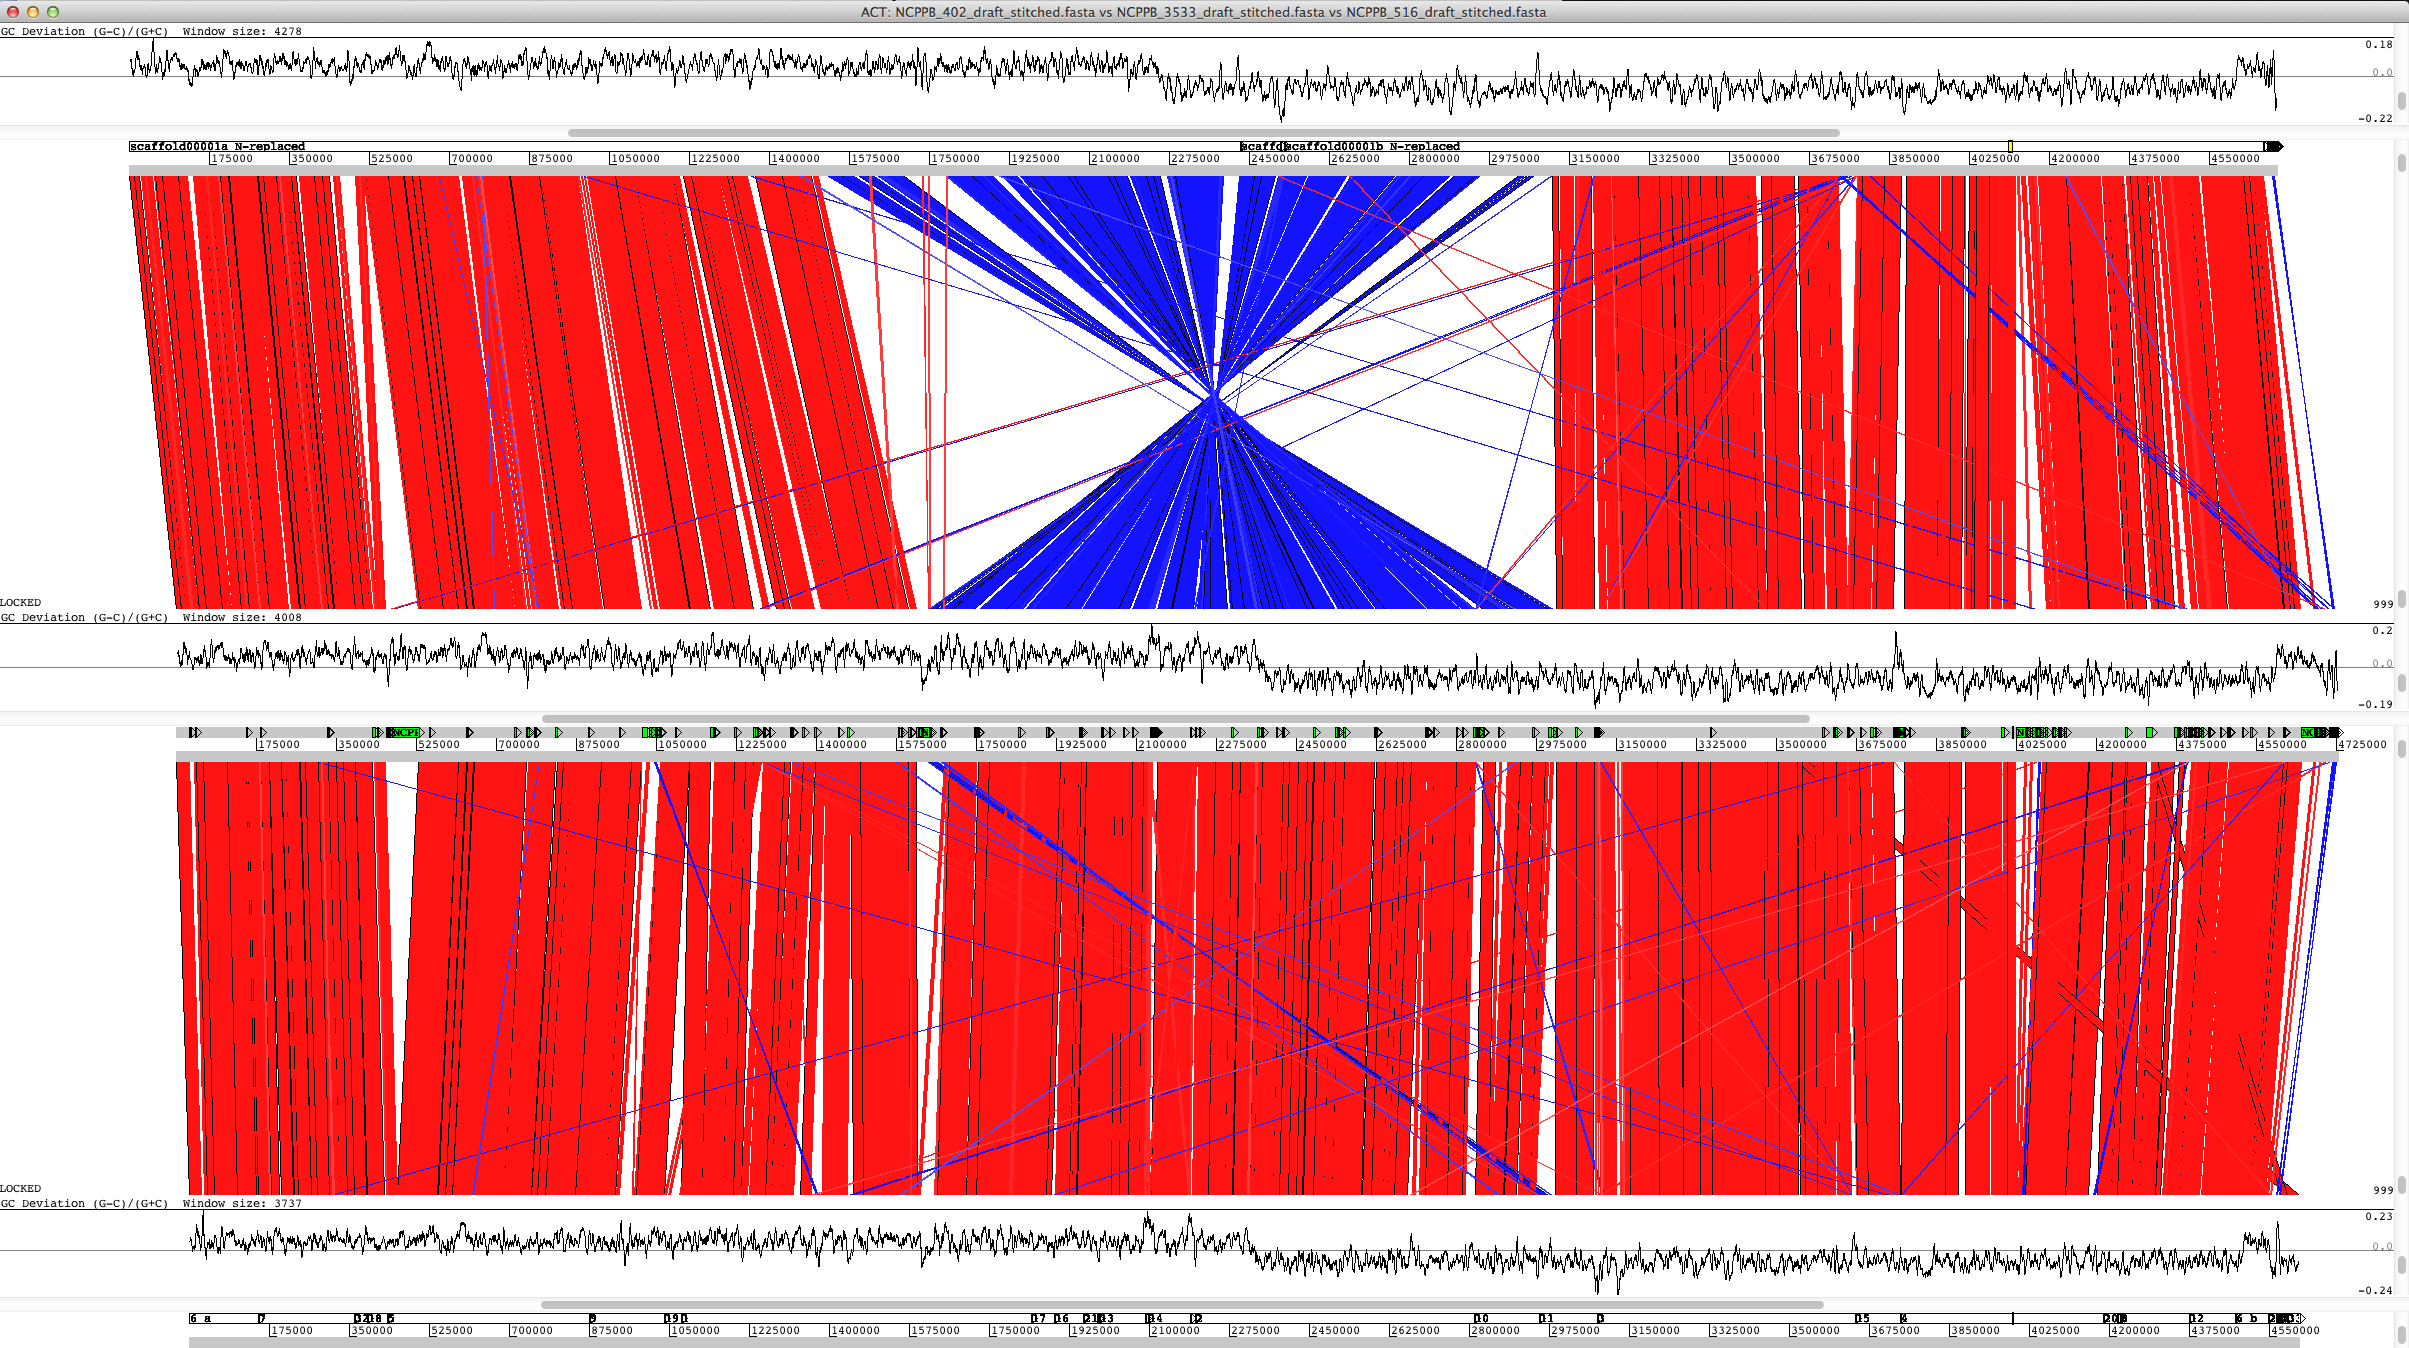
\includegraphics[width=0.6\textwidth]{images/act_comparison}
  \end{center}  
\end{frame}

% How do you align, and why?
\begin{frame}
  \frametitle{How to align, and why?}
  For useful analysis, the aligned genomes should:
  \begin{itemize}
    \item derive from a sufficiently recent common ancestor, so homologous regions can be identified
    \item derive from a sufficiently distant common ancestor, so that there are ``interesting'' differences to be identified
    \item \textbf{help to answer your biological question}: is your question organism or phenotype-specific? 
  \end{itemize}
  \begin{center}
    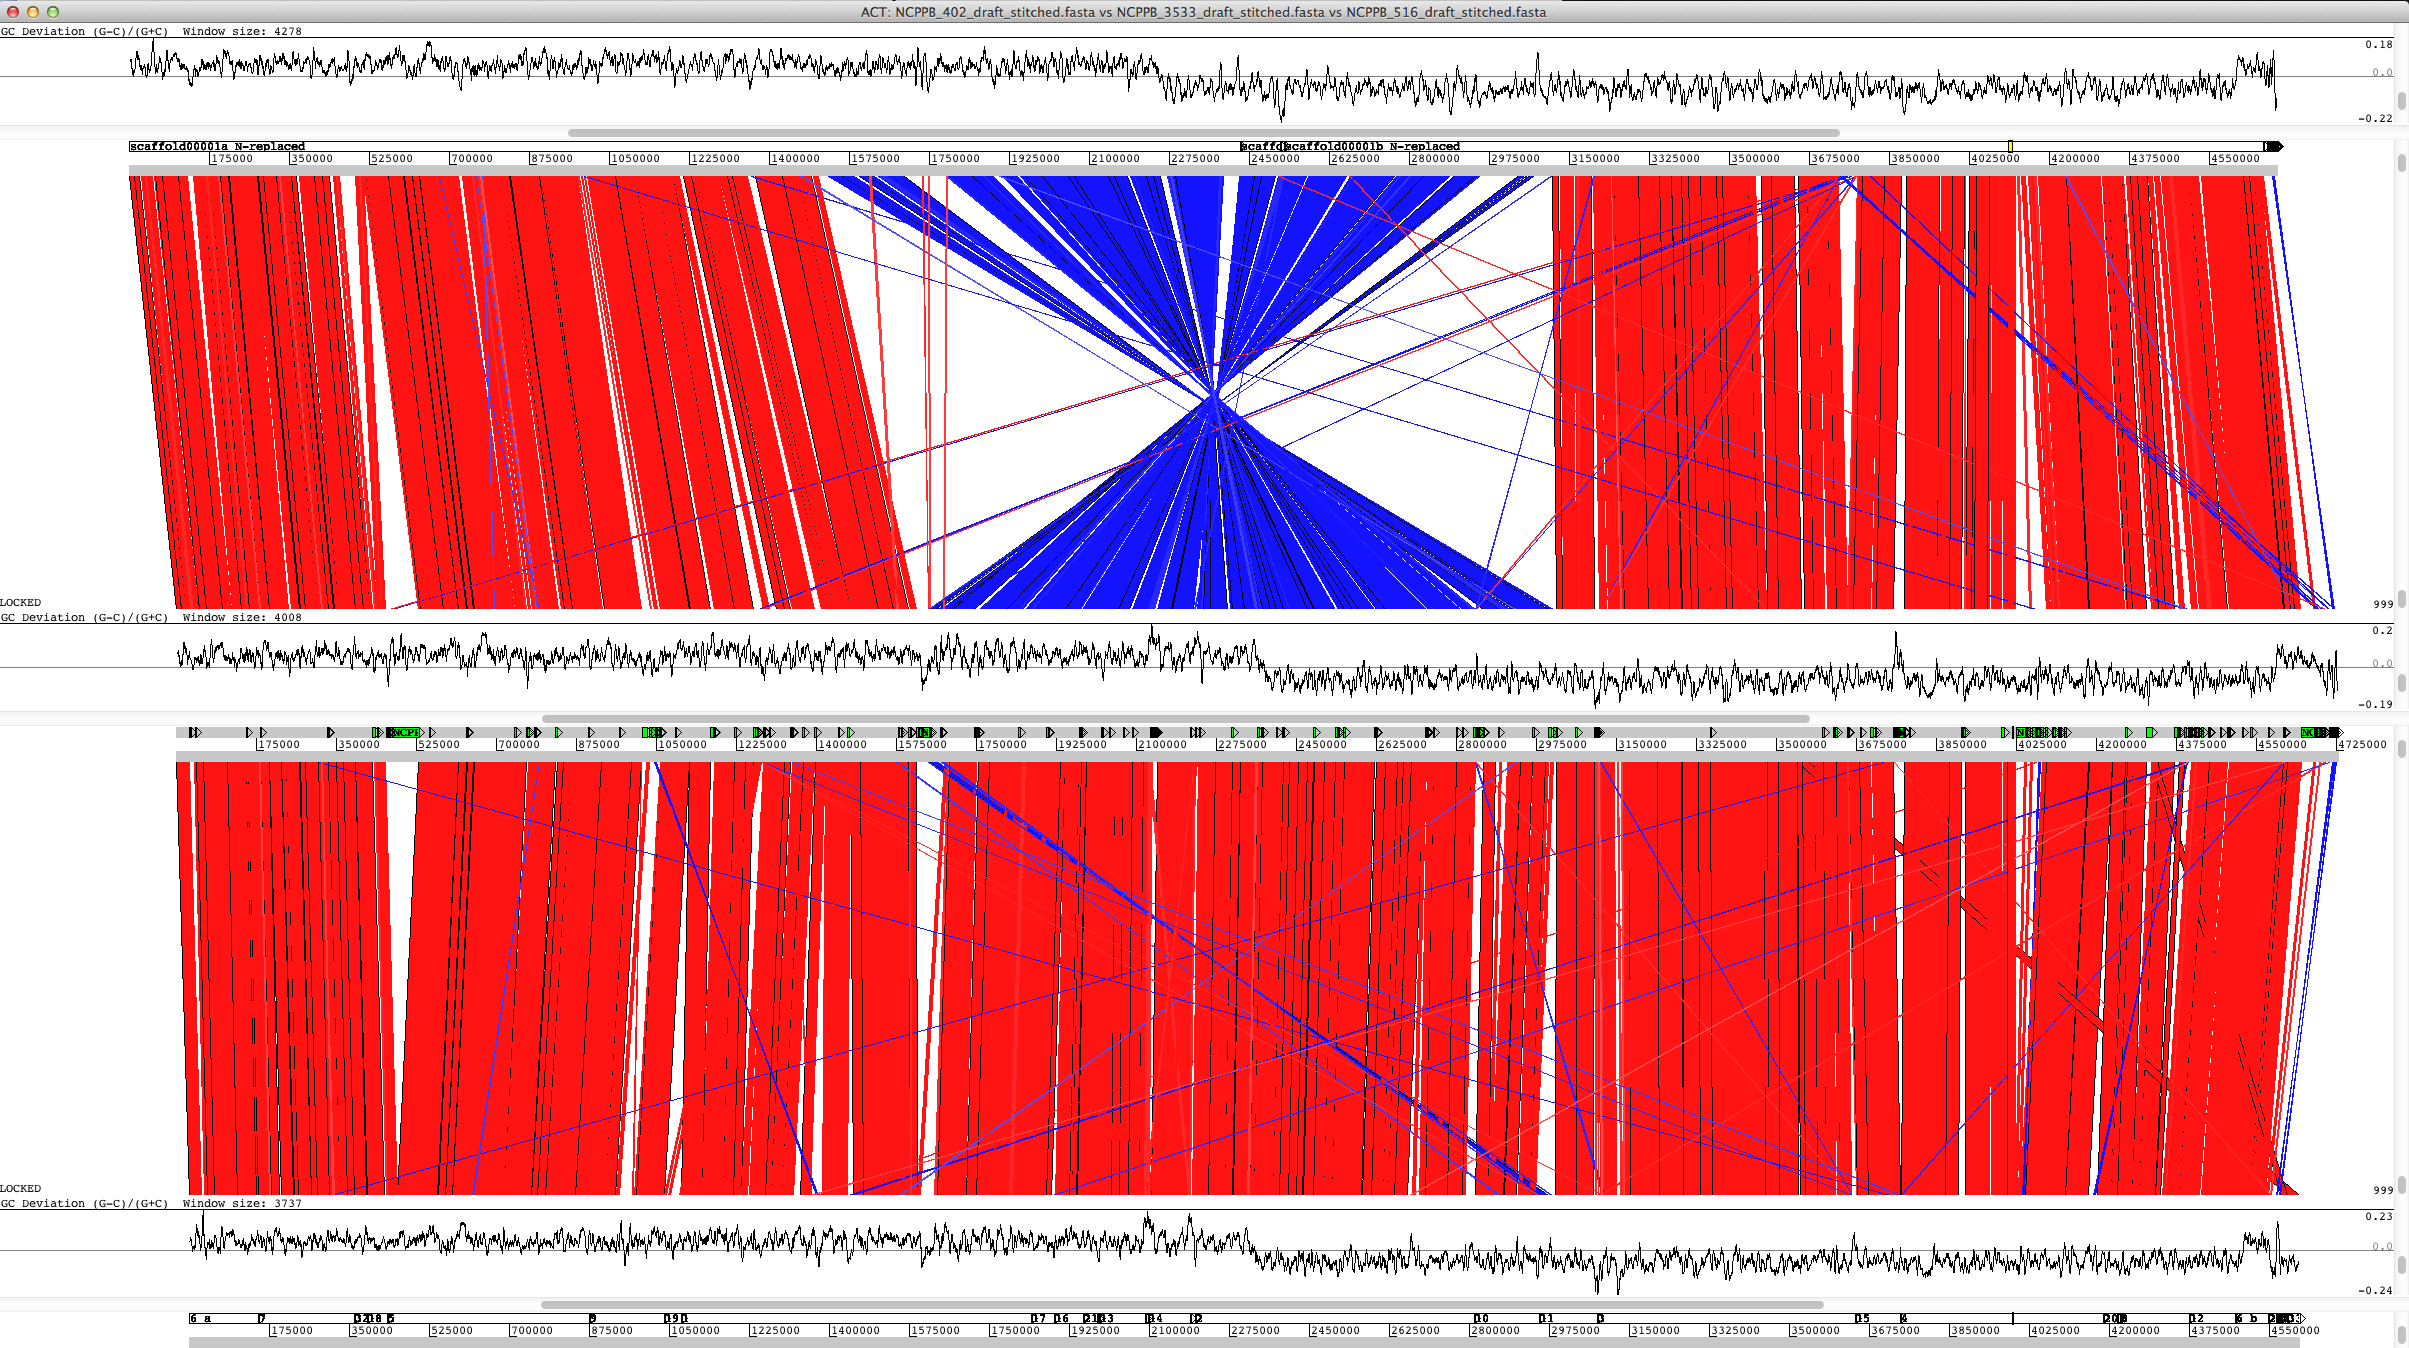
\includegraphics[width=0.6\textwidth]{images/act_comparison}
  \end{center}  
\end{frame}


% SUBSECTION: Average Nucleotide Identity
\subsection{Average Nucleotide Identity}

% DNA-DNA hybridisation
\begin{frame}
  \frametitle{DNA-DNA hybridisation\footnote{\tiny{\href{http://dx.doi.org/10.1016/S0168-6445(00)00040-1}{Morello-Mora and Amann (2001) \textit{FEMS Micro. Rev.} \textbf{25}:39-67 doi:10.1016/S0168-6445(00)00040-1}}}}
  \begin{columns}[T]
    \begin{column}{5cm}
      \begin{itemize}
        \item Denature DNA from two organisms.
        \item Allow to anneal. Reassociation $\approx$ similarity, measured as $\Delta T$  of denaturation curves.
        \item Proxy for sequence similarity.
        \item ``Gold Standard'' for prokaryotic taxonomy, since 1960s. ``70\% identity $\approx$ same species.''
      \end{itemize}
    \end{column}
    \begin{column}{5cm}
      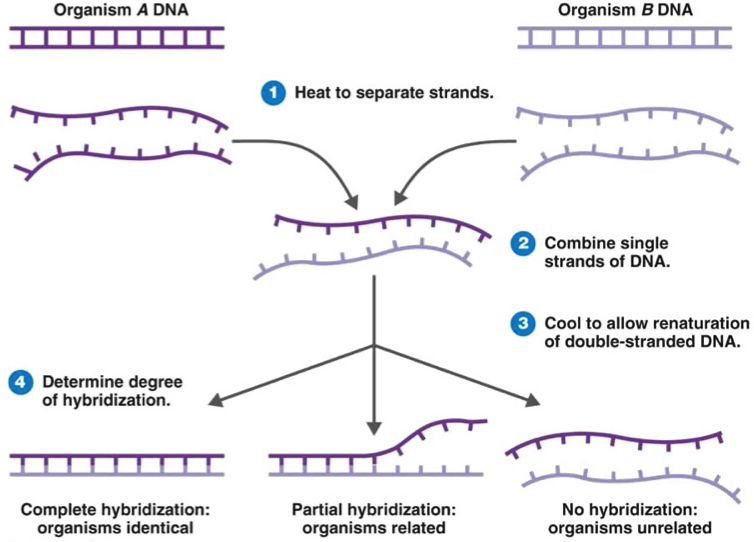
\includegraphics[width=1\textwidth]{images/ddh}
    \end{column}
  \end{columns}
\end{frame}

% ANIb
\begin{frame}
  \frametitle{Average Nucleotide Identity (ANIb)\footnote{\tiny{\href{http://dx.doi.org/10.1099/ijs.0.64483-0}{Goris \textit{et al}. (2007) \textit{Int. J. Syst. Biol.} \textbf{57}:81-91 doi:10.1099/ijs.0.64483-0}}}}
  \begin{columns}[T]
    \begin{column}{5cm}
      1. Break genomes into 1020t fragments\\
      2. \textbf{ANIb}: Mean \% identity of all BLASTN matches with $>30\%$ identity and $>70\%$ fragment coverage.\\[0.5cm]
      \begin{itemize}
        \item DDH:ANIb linear
        \item DDH:\%ID linear
        \item 70\%ID $\approx$ 95\%ANIb
      \end{itemize}
    \end{column}
    \begin{column}{5cm}
      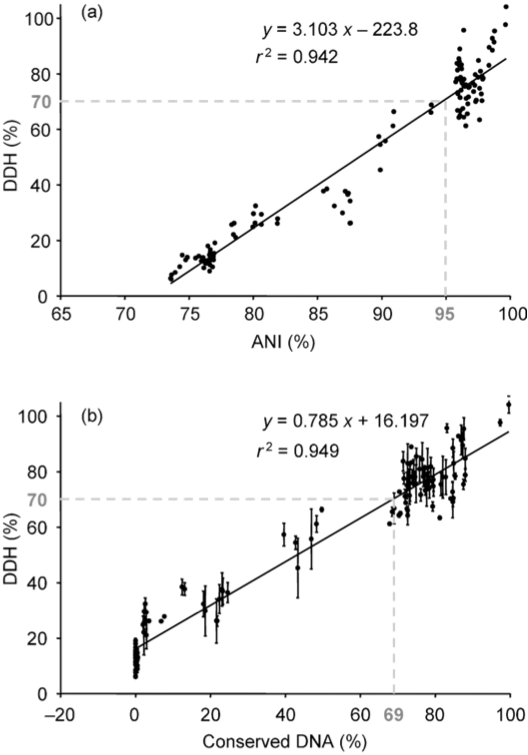
\includegraphics[width=1\textwidth]{images/ddh_ani_pid}
    \end{column}
  \end{columns}
\end{frame}

% ANIm
\begin{frame}
  \frametitle{Average Nucleotide Identity (ANIm)\footnote{\tiny{\href{http://dx.doi.org/10.1073/pnas.0906412106}{Richter and Rossello-Mora (2009) \textit{Proc. Natl. Acad. Sci. USA} \textbf{106}:19126-19131 doi:10.1073/pnas.0906412106}}}}
  \begin{columns}[T]
    \begin{column}{3cm}
      1. Align genomes with MUMmer\\
      2. \textbf{ANIm}: Mean \% identity of all matches\\[0.25cm]
      \begin{itemize}
        \item DDH:ANIm linear
        \item 70\%ID $\approx$ 95\%ANIb
      \end{itemize}
    \end{column}
    \begin{column}{7cm}
      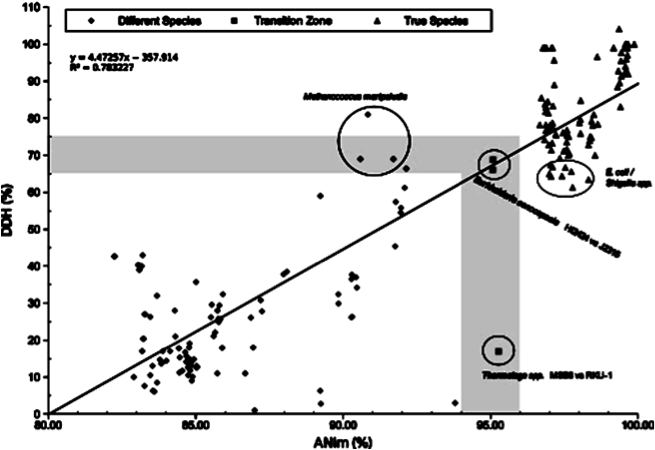
\includegraphics[width=1\textwidth]{images/ddh_anim}
    \end{column}
  \end{columns}
  \textbf{TETRA}: tetranucleotide frequency-based classifier introduced in same paper.
\end{frame}

% ANIb/ANIm/TETRA comparison
\begin{frame}
  \frametitle{ANI/TETRA comparison}
  All three methods applied to \textit{Anaplasma} spp.\\[0.25cm]
  \begin{columns}[T]
    \begin{column}{4cm}
    ANIb:\\
      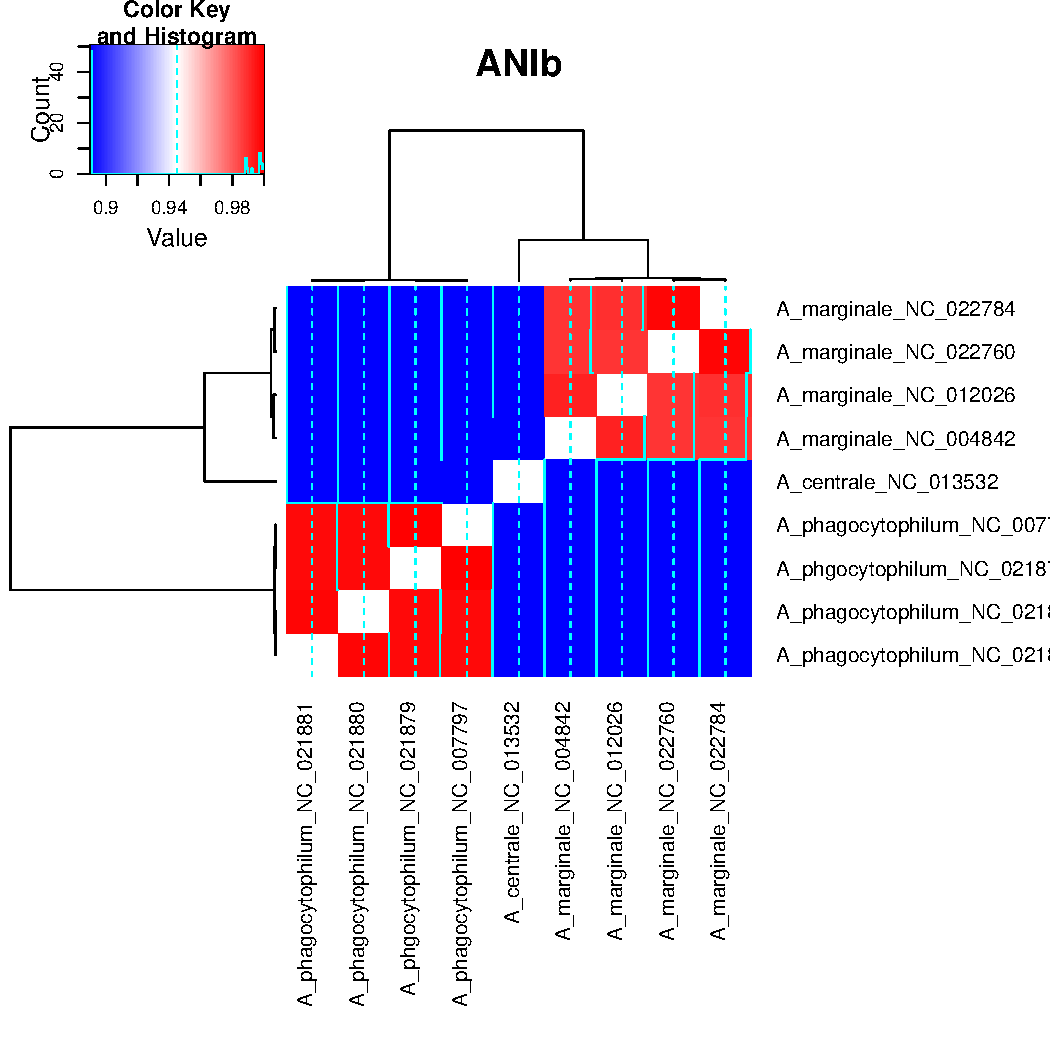
\includegraphics[width=1\textwidth]{images/ANIb}
    \end{column}
    \begin{column}{4cm}
    ANIm:\\
      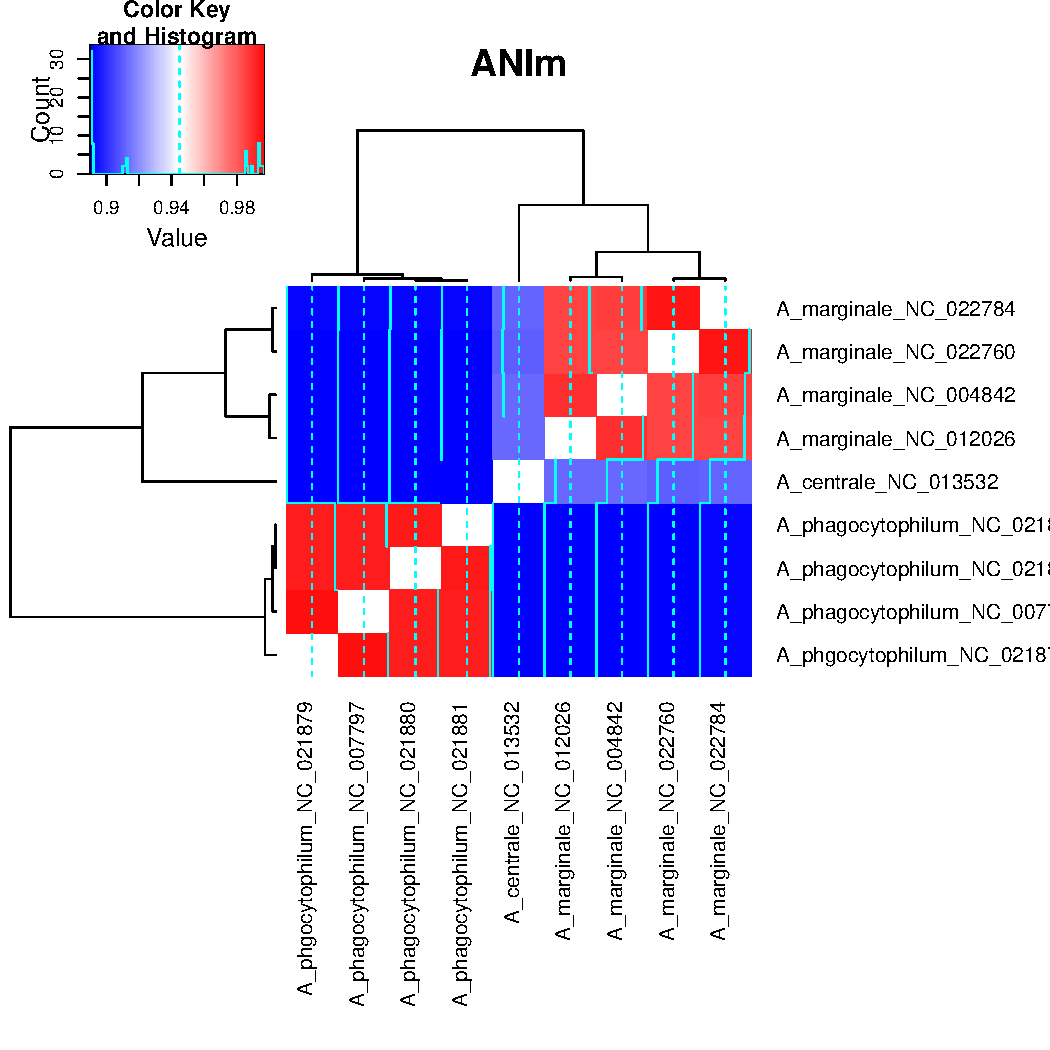
\includegraphics[width=1\textwidth]{images/ANIm}
    \end{column}
    \begin{column}{4cm}   
    TETRA:\\
      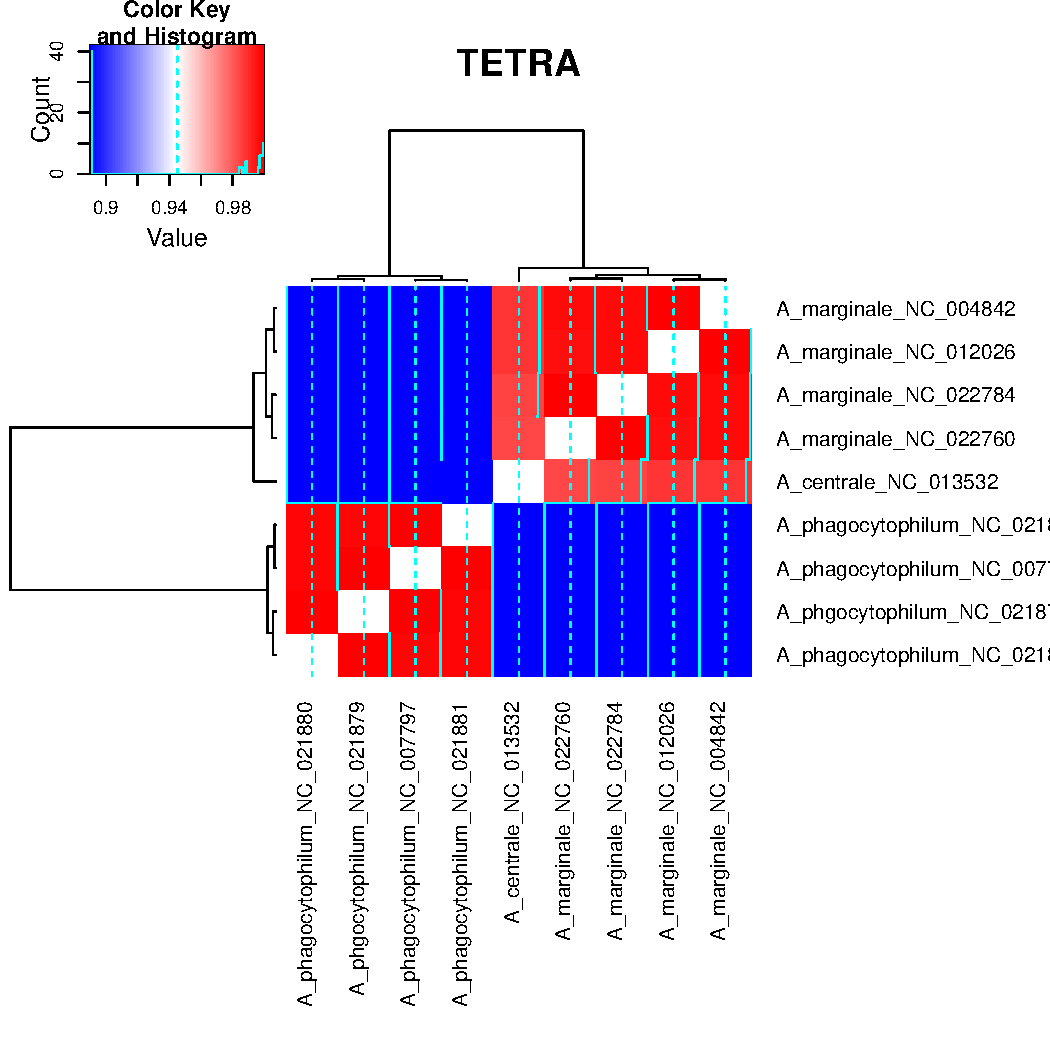
\includegraphics[width=1\textwidth]{images/TETRA}
    \end{column}
  \end{columns}       
  ANIb discards information, relative to ANIm\\
  ANIb/ANIm reflect evolutionary history; TETRA reflects bulk composition
\end{frame}

% ANIm in practice
\begin{frame}
  \frametitle{ANI in practice}
  Two practical applications\\[0.25cm]
  \begin{columns}[T]
    \begin{column}{6cm}
    29 \textit{Dickeya} isolates:\\
    More complex species structure\\
      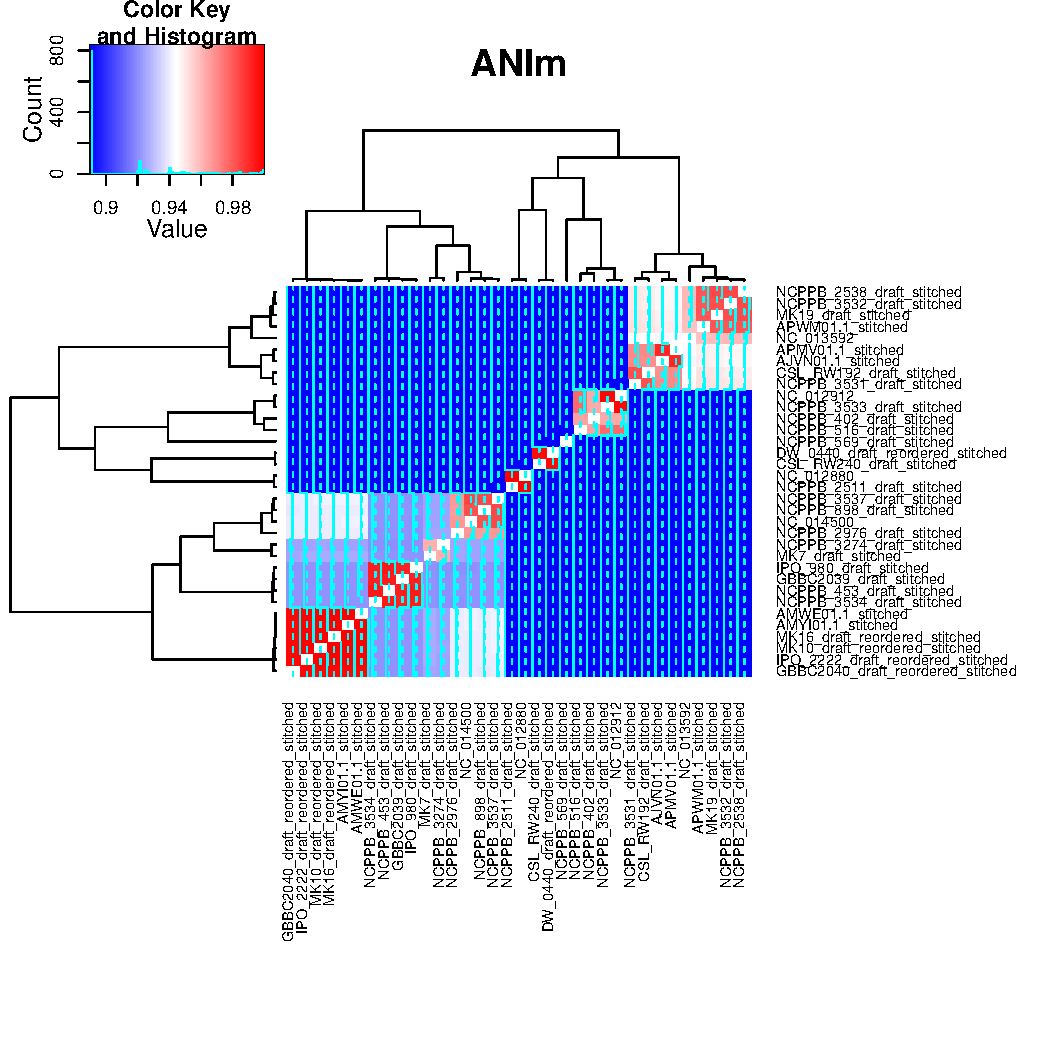
\includegraphics[width=1\textwidth]{images/ANIm_Dickeya}
    \end{column}
    \begin{column}{6cm}
    180 \textit{E.coli} isolates:\\
    More complex subtyping
      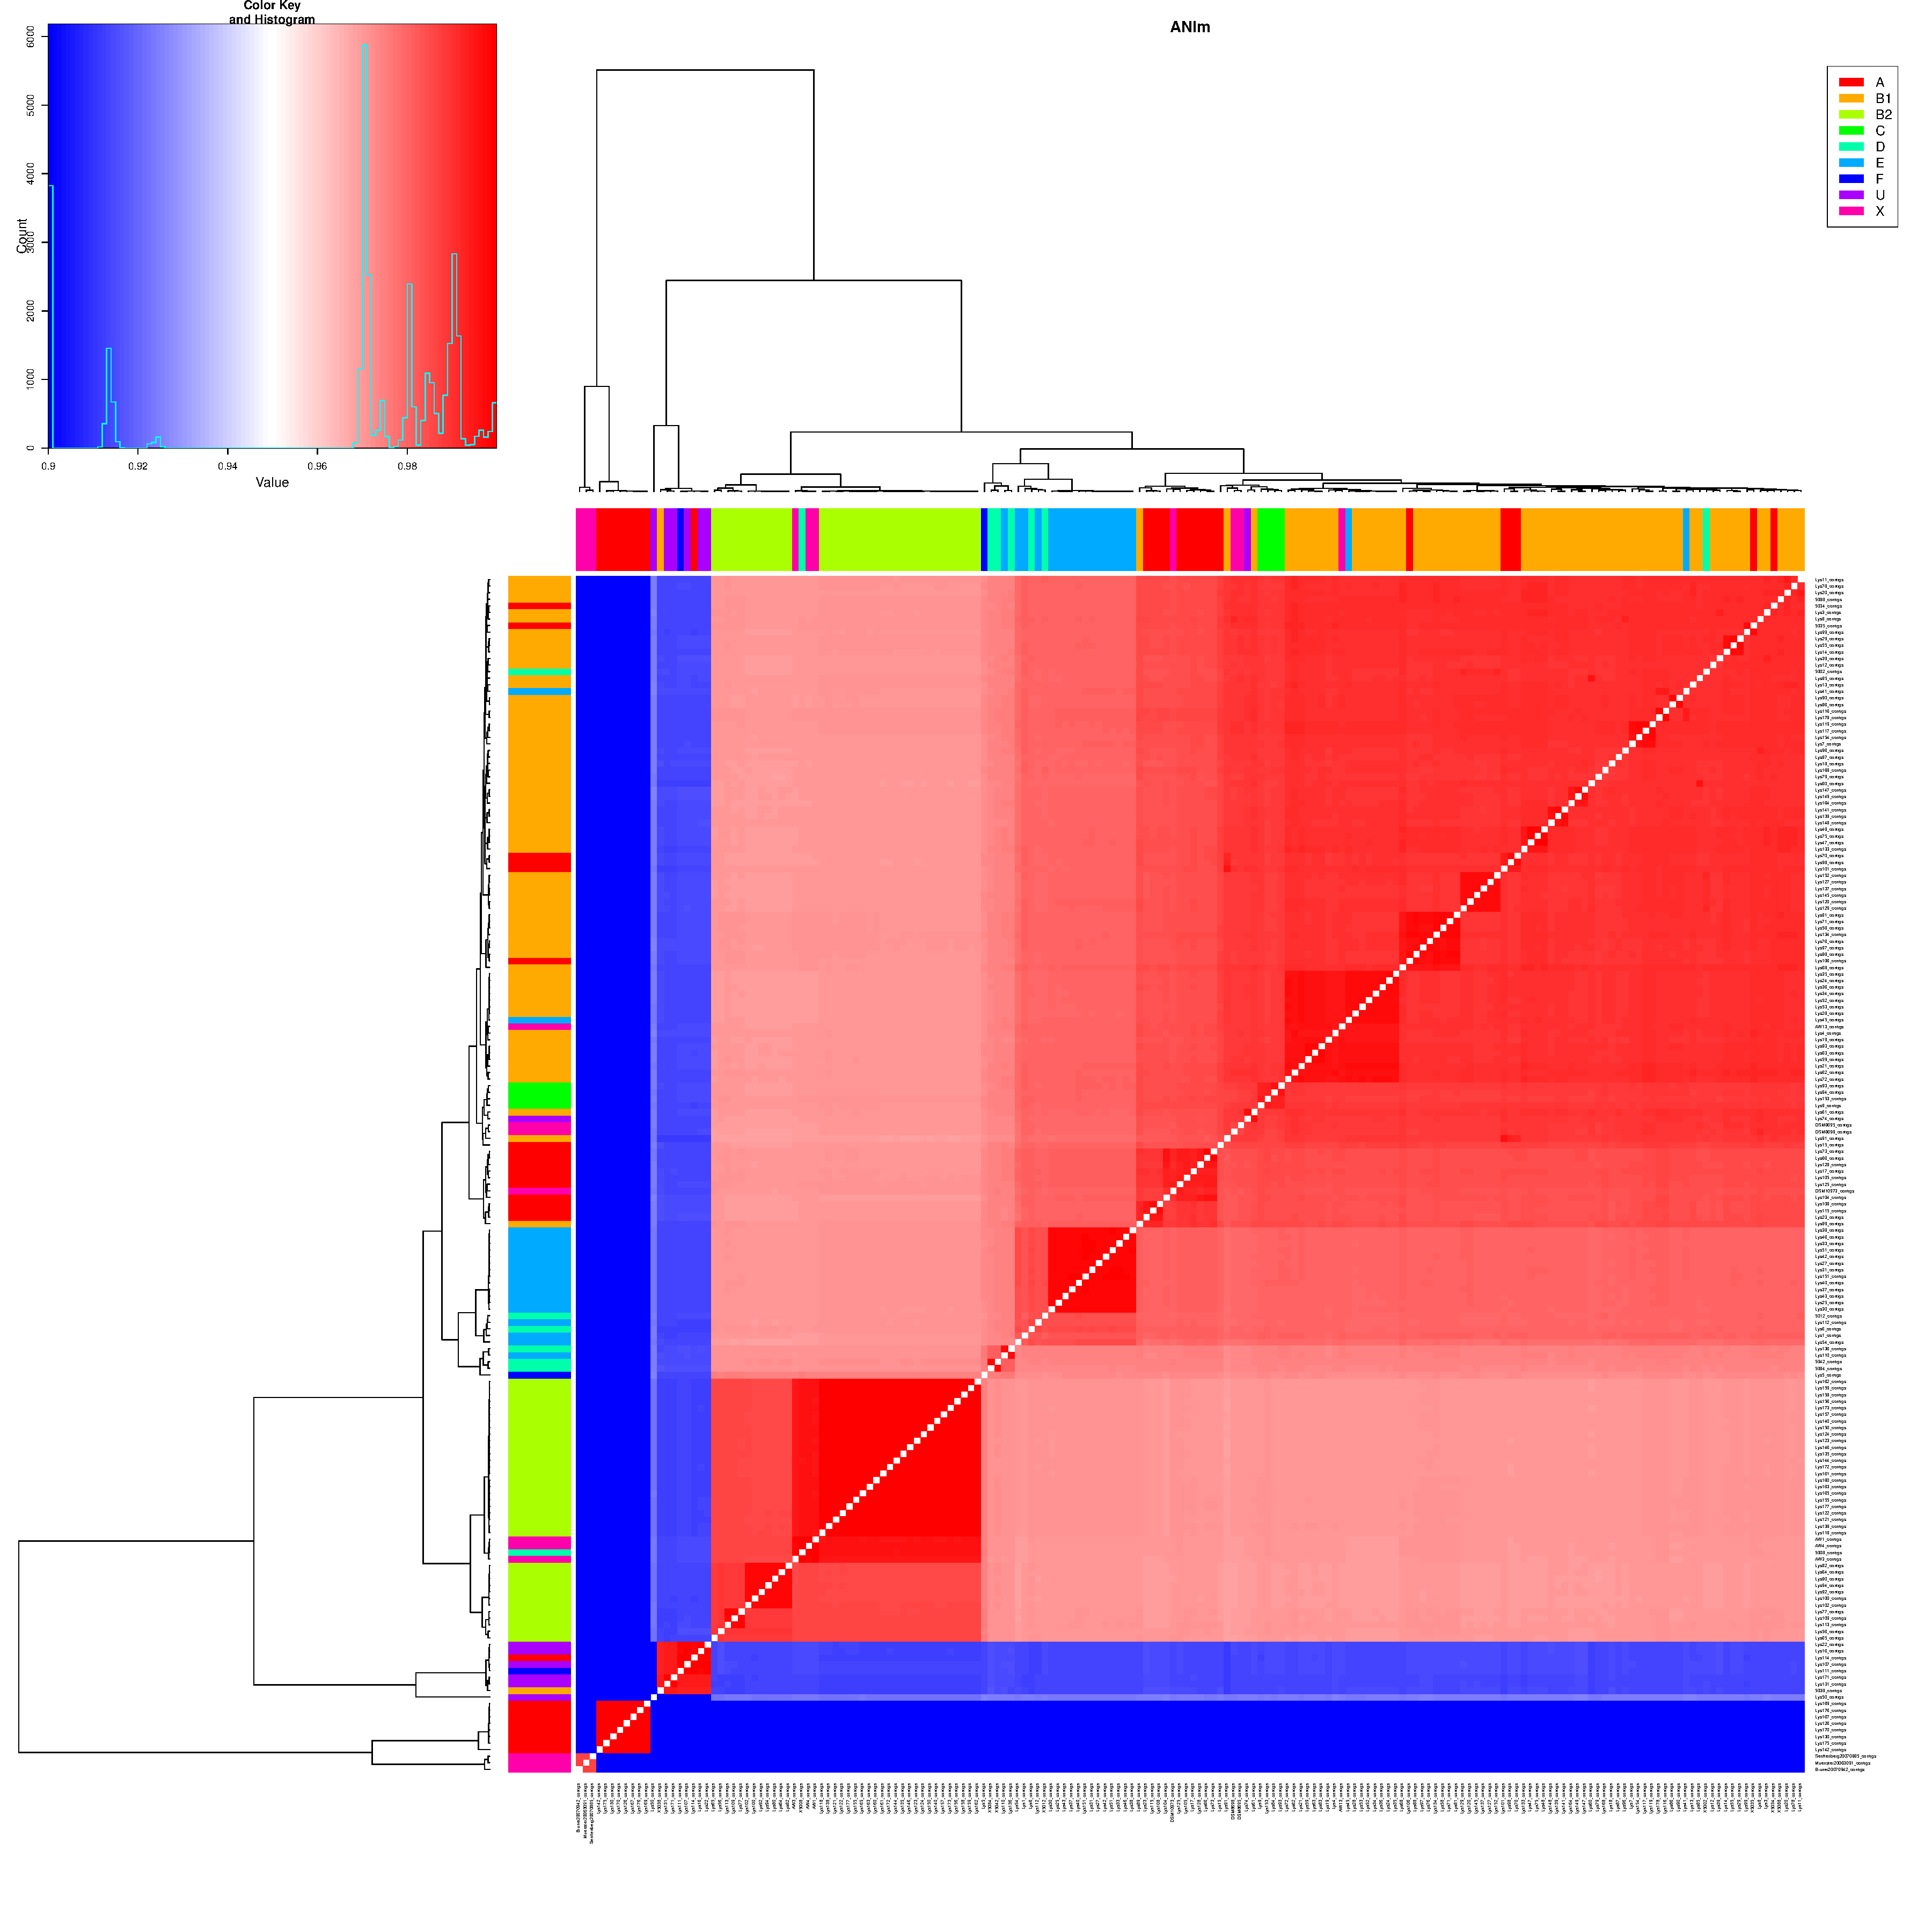
\includegraphics[width=1\textwidth]{images/ANIm_Ecoli}
    \end{column}
  \end{columns}       
\end{frame}